% ==============================================================================
% Section 5: Analytical Properties and System Bounds
% ==============================================================================

\section{Analytical Properties and System Bounds}
\label{sec:theoretical_invariants}

Hybrid models that couple discrete agent states with continuous reaction-diffusion-advection partial differential equations (PDEs) require explicit energy-accounting bounds and dynamical consistency conditions. Unconstrained agent update rules can violate carrying-capacity bounds or obscure the timescale separation between grazing depletion and biochemical induction. This section establishes three analytical properties of the model: bounded capacity and non-reproductive metabolic dissipation (Proposition~\ref{prop:capacity_boundedness}), the worst-case continuous-grazing critical synthesis delay $\theta_{\mathrm{crit}}$ (Proposition~\ref{thm:critical_synthesis_delay}), and the mean-field delay-bifurcation threshold $\tau^*$ (Proposition~\ref{thm:hopf_limit_cycle}). Double-buffered memory isolation and cross-thread reproducibility belong to the software implementation and are presented in Section~\ref{subsec:double_buffering_zarr}.

\begin{figure*}[t]
  \centering
  % ==============================================================================
% Figure 6: Analytical Invariant Boundaries and Bifurcation Surfaces
% Publication-Grade Vector Graphic (Springer Nature Two-Column Full-Width Spanning)
% ==============================================================================

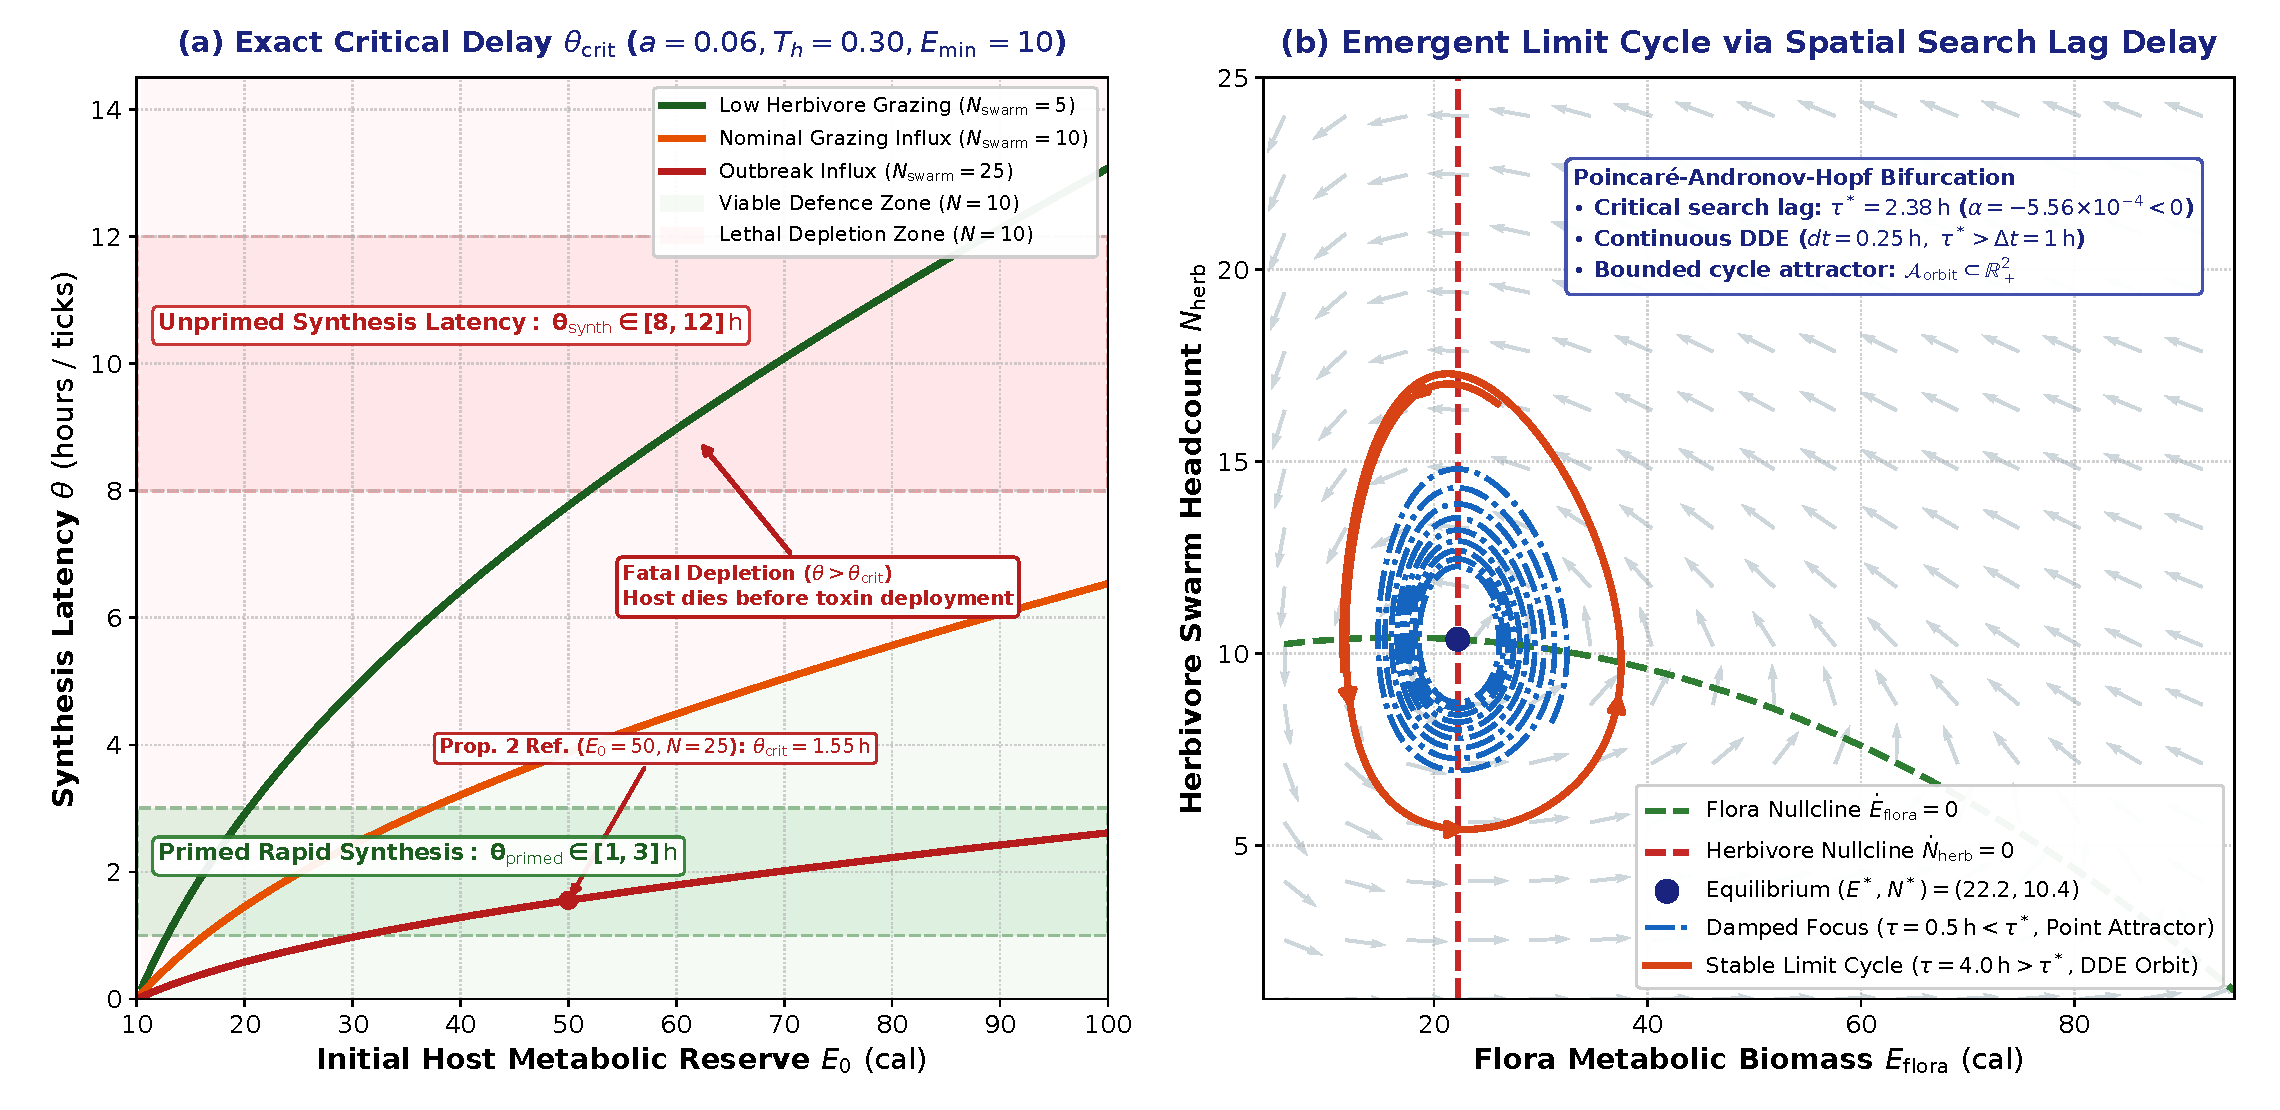
\includegraphics[width=0.92\textwidth]{figures/fig06_limit_cycle_bifurcation.pdf}

  \caption{Analytical Stability Boundaries and Mean-Field Delay Bifurcation Surfaces. (a) Critical synthesis latency bound $\theta_{\mathrm{crit}}$ as a function of initial host metabolic reserve $E_0$ and co-located grazing pressure $N_{\mathrm{swarm}}$ under continuous hourly intake. The shaded region separates the parameter zone in which pre-primed synthesis ($\theta_{\mathrm{primed}} < \theta_{\mathrm{crit}}$) preserves the host above $E_{\min}$ from the zone of lethal depletion. (b) Phase portrait in the $(E_{\mathrm{flora}}, N_{\mathrm{herb}})$ plane for the time-scaled delayed Rosenzweig--MacArthur system ($r = 0.02\,\mathrm{h}^{-1}$, $a = 0.002\,\mathrm{cell}^{-1}\mathrm{h}^{-1}$, $T_h = 7.5\,\mathrm{h}$, $e_{\mathrm{eff}} = 0.60$, $m_{\mathrm{herb}} = 0.02\,\mathrm{h}^{-1}$, $K = 100.0\,\mathrm{cal}$), illustrating convergence to a damped focus at $\tau = 0.5\,\mathrm{h} < \tau^*$ and a bounded limit cycle $\mathcal{A}_{\mathrm{orbit}}$ at $\tau = 4.0\,\mathrm{h} > \tau^* = 2.38\,\mathrm{h}$.}
  \label{fig:limit_cycle_bifurcation}
\end{figure*}

% ==============================================================================
\subsection{Capacity Bound and Non-Reproductive Dissipation}
\label{subsec:thermodynamic_conservation}
% ==============================================================================

Let $\mathcal{E}_t^{\mathrm{flora}} \subseteq \Lambda$ denote the set of active plant entities (at most one per lattice coordinate $(x, y) \in \Lambda$, carrying energy $E_i(t) \in [0, E_{\max}]$) and $\mathcal{S}_t^{\mathrm{herb}}$ the active herbivore swarms ($E_j^{\mathrm{herb}}(t) \le E_{\max}^{\mathrm{swarm}}$, bounded per tile by $C_{\max}$ so global swarm count satisfies $|\mathcal{S}_t^{\mathrm{herb}}| \le |\Lambda| C_{\max}$). Aggregate active somatic and swarm energy is defined as:
\begin{equation}
  \mathcal{H}_{\mathrm{biotope}}(t) \coloneqq \sum_{i \in \mathcal{E}_t^{\mathrm{flora}}} E_i(t) + \sum_{j \in \mathcal{S}_t^{\mathrm{herb}}} E_j^{\mathrm{herb}}(t).
  \label{eq:aggregate_energy_def}
\end{equation}

\begin{proposition}[Capacity Bound and Non-Reproductive Dissipation]
\label{prop:capacity_boundedness}
Under the coupled transition operators of PHIDS:
\begin{enumerate}
  \item \textbf{Capacity Ceiling:} For all ticks $t \ge 0$, aggregate active energy remains bounded by finite lattice capacity: $\mathcal{H}_{\mathrm{biotope}}(t) \le |\Lambda| E_{\max} + |\mathcal{S}_{\max}| E_{\max}^{\mathrm{swarm}} < \infty$.
  \item \textbf{Non-Reproductive Metabolic Dissipation:} On any tick without photosynthetic influx ($\Phi_{\mathrm{photo}}(t) = 0$) and without seedling germination events (or globally for parameterisations satisfying $E_{\mathrm{seed}} \ge E_{\mathrm{base}}$), net total energy is non-increasing, $\Delta \mathcal{H}_{\mathrm{biotope}}(t) \le -\Phi_{\mathrm{struct}}(t) - \Phi_{\mathrm{myco}}(t) - \Phi_{\mathrm{resp}}(t) - \Phi_{\mathrm{def}}(t) - \Phi_{\mathrm{waste}}(t) \le 0$, with strict dissipation ($\Delta \mathcal{H}_{\mathrm{biotope}}(t) < 0$) whenever mature structural flora ($M_i > 0$), active herbivores, active inducible defences, or mycorrhizal links exist on the evaluated step.
\end{enumerate}
\end{proposition}

\begin{proof}
Because at most one plant occupies each grid cell, $|\mathcal{E}_t^{\mathrm{flora}}| \le |\Lambda|$, and growth saturates via $E_i(t+1) = \min(E_{\max}, E_i(t) + \Delta E_{\mathrm{growth},i})$. Swarm occupancy per cell is masked at capacity $C_{\max}$ and binary fission halves parent energy ($E_{\mathrm{child}} = E_{\mathrm{parent}}/2$), establishing Part~1. For Part~2, grazing extracts $\Delta E_{\mathrm{grazed}}$ with net assimilated fraction $\tilde{e}_{\mathrm{eff}} = (1 - \delta_{\mathrm{morph}}) e_{\mathrm{eff}} \in (0, 1)$, dissipating $\Phi_{\mathrm{waste}} = (1 - \tilde{e}_{\mathrm{eff}})\Delta E_{\mathrm{grazed}} \ge 0$; enzyme synthesis deducts $\Phi_{\mathrm{def}} = \sum c_{\mathrm{synth}} \ge 0$, mycorrhizal establishment and weekly link upkeep deduct $\Phi_{\mathrm{myco}} \ge 0$, plant cohorts with $M_i > 0$ deduct structural maintenance $\Phi_{\mathrm{struct}} = \sum 0.5\,E_{\min}\,(M_i / M_{\max}) \ge 0$, and diurnal active herbivores deduct basal respiration $\Phi_{\mathrm{resp}} \ge 0$ (while resetting negative energy after integer starvation deductions via Eq.~\eqref{eq:integer_casualty_clearing}). Setting $\Phi_{\mathrm{photo}} = 0$ leaves $\Delta \mathcal{H}_{\mathrm{biotope}} \le 0$ whenever germination either adds no energy ($E_{\mathrm{seed}} \ge E_{\mathrm{base}}$) or is absent on the step, and strictly negative whenever any dissipation channel acts (newly germinated seedlings carry $M_i = 0$ and zero links until their first active structural cohort). When parameterisations set $E_{\mathrm{base}} > E_{\mathrm{seed}}$ (Table~\ref{tab:case_study_configurations}), each germination introduces an establishment-carbon subsidy $E_{\mathrm{base}} - E_{\mathrm{seed}} > 0$ representing seedbank reserves, remaining globally bounded by Part~1.
\end{proof}

% ==============================================================================
\subsection{Continuous-Grazing Critical Synthesis Delay}
\label{subsec:critical_synthesis_delay}
% ==============================================================================

Unprimed plants incur a physiological synthesis delay $\theta_{\mathrm{synth}}$ --- encompassing elicitor perception, jasmonate signalling, and enzymatic translation --- before inducible toxins become active. Consider a single host plant with initial reserve $E_0 > E_{\min}$ at $t = 0$ subjected to a worst-case continuous per-tick feeding regime (applying the per-event functional response Eq.~\eqref{eq:math_holling_type_ii} at every hourly step $\Delta t = 1\,\text{h}$ with movement period $v = 1$, rather than on $24$-tick diurnal strides) by a co-located swarm of size $N_{\mathrm{swarm}}$:
\begin{equation}
  \dot{E}_{\mathrm{loss}}(E) = \frac{a E}{1 + a T_h E} \cdot N_{\mathrm{swarm}},
  \label{eq:intake_ode}
\end{equation}
where $a$ is the effective per-event attack rate and $T_h$ the handling time per unit biomass. Unprimed hosts experience $\theta_{\mathrm{synth}} \in [8, 12]\,\text{h}$ without chemical deterrence ($\delta_{\mathrm{chem}} = 0$) over $t \in [0, \theta_{\mathrm{synth}})$. If $E(t)$ falls below $E_{\min}$ prior to deployment, $\mathcal{T}_{\text{interact}}$ removes the host before toxins take effect. Eq.~\eqref{eq:intake_ode} defines a worst-case continuous-grazing lower bound corresponding to sustained hourly multi-swarm arrival; under $24$-tick diurnal strides, single-swarm grazing buffers moderate delays ($\theta_{\mathrm{synth}} \le 24\,\text{h}$) unless the initial grazing event depletes the host below $E_{\min}$.

\begin{proposition}[Continuous-Grazing Critical Synthesis Delay $\theta_{\mathrm{crit}}$]
\label{thm:critical_synthesis_delay}
Let a host plant have initial reserve $E_0 > E_{\min}$ under continuous hourly grazing governed by \eqref{eq:intake_ode}. The closed-form critical synthesis delay threshold $\theta_{\mathrm{crit}}$ separating host survival from deterministic mortality is:
\begin{equation}
  \theta_{\mathrm{crit}} \coloneqq \frac{1}{N_{\mathrm{swarm}}} \left[ \frac{1}{a} \ln\left(\frac{E_0}{E_{\min}}\right) + T_h (E_0 - E_{\min}) \right].
  \label{eq:theta_crit_exact}
\end{equation}
Accordingly:
\begin{enumerate}
  \item If $\theta_{\mathrm{synth}} > \theta_{\mathrm{crit}}$, unprimed host mortality occurs deterministically at $t^* = \theta_{\mathrm{crit}}$ prior to toxin deployment.
  \item If priming compresses synthesis latency to $\theta_{\mathrm{primed}} < \theta_{\mathrm{crit}}$, inducible defences activate before $E(t)$ reaches $E_{\min}$.
\end{enumerate}
\end{proposition}

\begin{proof}
Separating variables in $\frac{dE}{dt} = -\frac{a E}{1 + a T_h E} N_{\mathrm{swarm}}$ and integrating from $E(0) = E_0$ to $E(t)$ gives:
\begin{equation}
  \frac{1}{a} \ln\left(\frac{E(t)}{E_0}\right) + T_h \left(E(t) - E_0\right) = - N_{\mathrm{swarm}} \cdot t.
  \label{eq:integrated_depletion}
\end{equation}
Setting $E(t^*) = E_{\min}$ yields $t^* \equiv \theta_{\mathrm{crit}}$ directly as in \eqref{eq:theta_crit_exact}.
\end{proof}

\begin{remark}[Baseline Priming Regime]
For a reference host parameterised at $E_0 = 50\,\text{cal}$, $E_{\min}=10\,\text{cal}$, $a=0.06\,\text{cell}^{-1}\text{h}^{-1}$, and $T_h=0.30\,\text{h}$ under sustained grazing ($N_{\mathrm{swarm}} \geq 5$), nominal unprimed delays ($\theta_{\mathrm{synth}} \in [8, 12]\,\text{h}$) exceed $\theta_{\mathrm{crit}}$ (Fig.~\ref{fig:limit_cycle_bifurcation}a), whereas primed delays $\theta_{\mathrm{primed}} \in [1, 3]\,\text{h}$ lie inside the survival region across low to moderate swarm densities.
\end{remark}

% ==============================================================================
\subsection{Mean-Field Delay-Bifurcation Criterion}
\label{subsec:hopf_limit_cycle}
% ==============================================================================

Lumped predator--prey ODEs \cite{rosenzweig1963graphical} assume instantaneous spatial encounter. In lattice biotopes, herbivores incur finite transit lag moving between host patches as well as trophic assimilation lag. To isolate how spatial-trophic delay alters local stability in the undefended baseline prior to inducible defences, we project the baseline consumer--resource interaction onto a continuous-time mean-field delay differential equation (DDE) system:
\begin{align}
  \frac{dE}{dt} &= r E(t) \left(1 - \frac{E(t)}{K}\right) - \frac{a E(t)}{1 + a T_h E(t)} N(t), \label{eq:dde_flora} \\
  \frac{dN}{dt} &= e_{\mathrm{eff}} \frac{a E(t - \tau)}{1 + a T_h E(t - \tau)} N(t) - m_{\mathrm{herb}} N(t), \label{eq:dde_herb}
\end{align}
where $\tau \coloneqq \tau_{\mathrm{lag}} > 0$ denotes the effective spatial-search and trophic assimilation lag ($\tau_{\mathrm{spatial}} = \bar{d}_{\mathrm{patch}} / v_{\mathrm{eff}}$ plus digestive assimilation delay) of the undefended Rosenzweig--MacArthur baseline. The non-trivial coexistence equilibrium $(E^*, N^*)$ satisfies $\frac{dE}{dt} = \frac{dN}{dt} = 0$:
\begin{align}
  E^* &= \frac{m_{\mathrm{herb}}}{a (e_{\mathrm{eff}} - m_{\mathrm{herb}} T_h)}, \label{eq:interior_equilibrium_e} \\
  N^* &= \frac{r}{a}\left(1 - \frac{E^*}{K}\right)(1 + a T_h E^*). \label{eq:interior_equilibrium_n}
\end{align}
Choosing realistic hourly growth and mortality rates ($r = 0.02\,\text{h}^{-1}$, $K = 100.0\,\text{cal}$, $a = 0.002\,\text{cell}^{-1}\text{h}^{-1}$, $T_h = 7.5\,\text{h}$, $e_{\mathrm{eff}} = 0.60$, $m_{\mathrm{herb}} = 0.02\,\text{h}^{-1}$), Eqs.~\eqref{eq:interior_equilibrium_e}--\eqref{eq:interior_equilibrium_n} yield $(E^*, N^*) = (22.22\,\text{cal}, 10.37)$ to the right of the Rosenzweig--MacArthur nullcline hump ($E_{\mathrm{hump}} = 16.67\,\text{cal}$), ensuring local asymptotic stability ($\alpha = -5.56 \times 10^{-4} < 0$) at $\tau = 0$ and a Hopf bifurcation above the engine step size at $\tau^* = 2.38\,\text{h} > \Delta t = 1.0\,\text{h}$ (Fig.~\ref{fig:limit_cycle_bifurcation}b).

\begin{proposition}[Mean-Field Delay-Bifurcation Criterion]
\label{thm:hopf_limit_cycle}
Let $E^* < K$ such that an interior equilibrium $(E^*, N^*)$ exists, and let the linearised Jacobian of \eqref{eq:dde_flora}--\eqref{eq:dde_herb} about $(E^*, N^*)$ be given by:
\begin{equation}
  J_0 = \begin{pmatrix} \alpha & -\beta \\ 0 & 0 \end{pmatrix}, \quad J_\tau = \begin{pmatrix} 0 & 0 \\ \gamma & 0 \end{pmatrix},
\end{equation}
with $\alpha = r\left(1 - \frac{2E^*}{K}\right) - \frac{a N^*}{(1 + a T_h E^*)^2}$, $\beta = \frac{a E^*}{1 + a T_h E^*}$, and $\gamma = \frac{e_{\mathrm{eff}} a N^*}{(1 + a T_h E^*)^2}$. When $p = -\alpha > 0$, there exists a critical delay $\tau^*$ such that:
\begin{enumerate}
  \item For $\tau < \tau^*$, $(E^*, N^*)$ is locally asymptotically stable.
  \item At $\tau = \tau^*$, a pair of simple conjugate eigenvalues crosses the imaginary axis transversally (Poincaré--Andronov--Hopf bifurcation).
  \item For $\tau > \tau^*$, $(E^*, N^*)$ is linearly unstable and a periodic orbit branch bifurcates at $\tau^*$.
\end{enumerate}
The critical delay is:
\begin{equation}
  \tau^* = \frac{1}{\omega_0} \arccos\left( \frac{\omega_0^2}{r_{\mathrm{delay}}} \right),
  \label{eq:tau_star_exact}
\end{equation}
where $\omega_0 = \sqrt{\frac{-p^2 + \sqrt{p^4 + 4 r_{\mathrm{delay}}^2}}{2}}$ is the positive root of $\omega^4 + p^2\omega^2 - r_{\mathrm{delay}}^2 = 0$ with $r_{\mathrm{delay}} = \beta \gamma$.
\end{proposition}

\begin{proof}
Linearising \eqref{eq:dde_flora}--\eqref{eq:dde_herb} yields the characteristic quasipolynomial $\mathcal{D}(\lambda, \tau) = \lambda^2 + p\lambda + r_{\mathrm{delay}} e^{-\lambda\tau} = 0$ ($p = -\alpha > 0$, $r_{\mathrm{delay}} = \beta\gamma > 0$). Substituting $\lambda = i\omega$ ($\omega > 0$) gives $\omega^2 = r_{\mathrm{delay}}\cos(\omega\tau)$ and $p\omega = r_{\mathrm{delay}}\sin(\omega\tau)$, eliminating $\tau$ to yield $\omega^4 + p^2\omega^2 - r_{\mathrm{delay}}^2 = 0$, unique positive root $\omega_0$, and $\tau^*$ in \eqref{eq:tau_star_exact}. Implicit differentiation at $\lambda = i\omega_0$ yields $\operatorname{Re}\!\left[\left.(d\lambda/d\tau)^{-1}\right|_{\tau=\tau^*}\right] = (2\omega_0^2 + p^2)/r_{\mathrm{delay}}^2 > 0$, verifying transversal crossing.
\end{proof}

\begin{remark}[Numerical Verification and Diagnostic Role]
At the time-scaled reference parameters above, numerical DDE integration (Fig.~\ref{fig:limit_cycle_bifurcation}b) confirms a damped spiral focus at $\tau = 0.5\,\mathrm{h} < \tau^*$ and convergence onto a bounded limit cycle $\mathcal{A}_{\mathrm{orbit}} \subset \mathbb{R}_+^2$ at $\tau = 4.0\,\mathrm{h} > \tau^* = 2.38\,\mathrm{h}$. In calibrated multi-species runs where $E^* < E_{\mathrm{hump}}$ ($\alpha > 0$ at $\tau = 0$; Section~\ref{sec:ecotone_theorem_parity}), the lumped DDE prerequisite $p > 0$ is violated, diagnosing that coexistence depends on spatial dispersal and multi-guild resource partitioning rather than local ODE equilibrium stability.
\end{remark}
